% 图 51.3 —— 由 `checks/emit_hand.py` 自动拼出（probe 精测 + prims2 图元分解）
%%
% ⚠ 这是**稿子不是成品**：跑 `checks/checkhand.py 51.3` 看指标 + 看叠合图。
%%
%% ⚠ 待核：
%   · 本图 probe 报出阴影族 1 个 —— **本脚本不生成阴影**（要照原书手写）；prims2 的 strokes 里可能含阴影线，核对时留意别画重
%   · 可疑字形 1 项（空心圈 ⊙ 常被认成字母 o）—— 见文件末
%%
\documentclass[12pt]{standalone}
\usepackage{fontspec}
\setsansfont{Arial}
\newfontfamily\mfallback{DejaVu Sans}
\usepackage{tikz}
\begin{document}
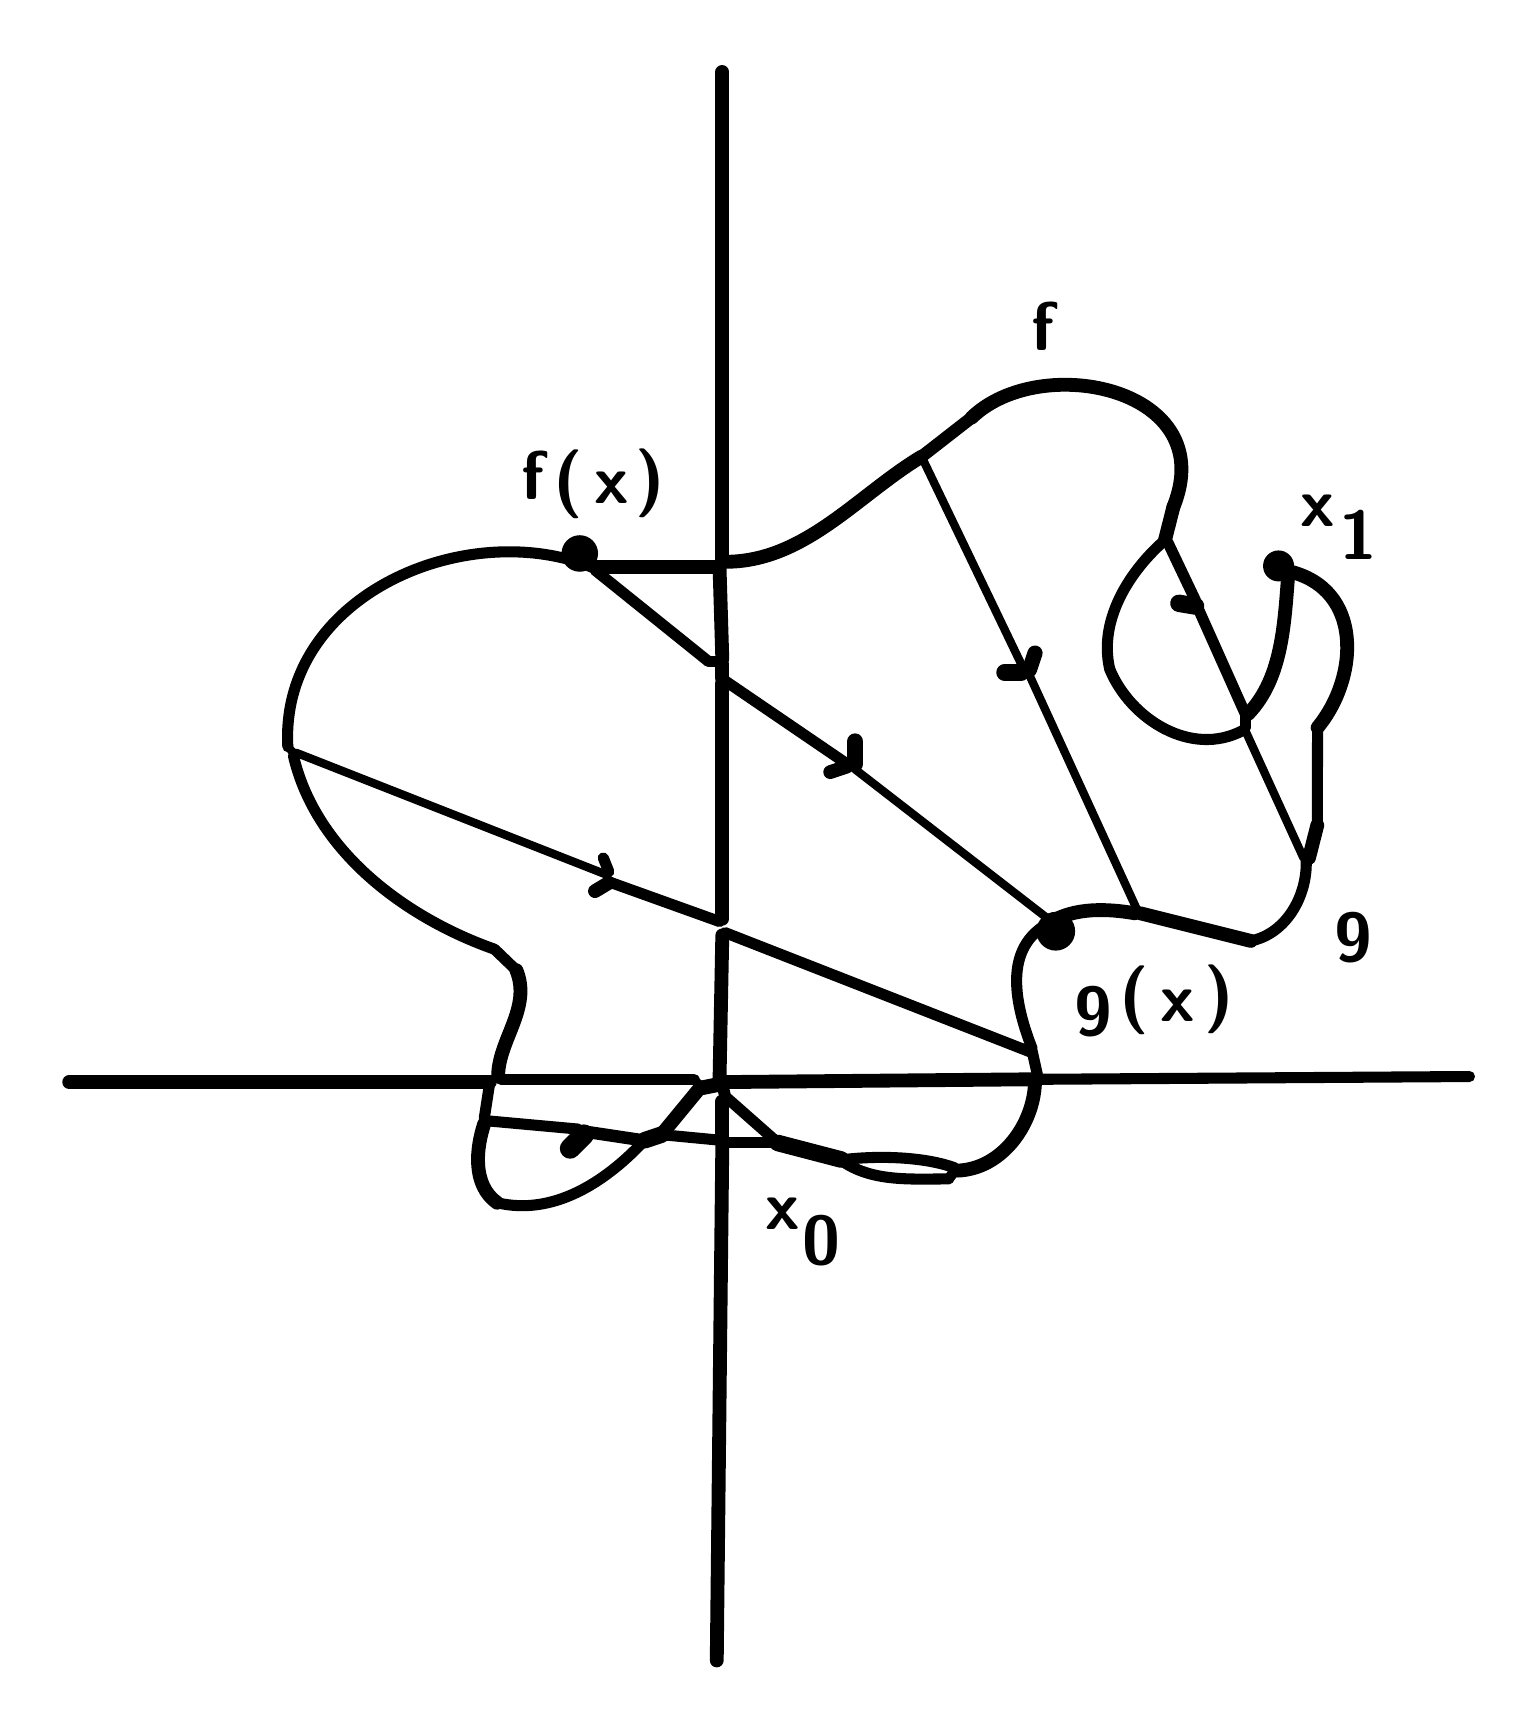
\begin{tikzpicture}[x=1pt, y=-1pt, line width=3.0pt, line cap=round, line join=round]

  %% ════ 填充区（prims2 的 fills）════

  %% ════ 直线段（prims2 的 strokes）════
  \draw[line width=3.0pt] (440.0,254.0) -- (461.0,300.0);
  \draw[line width=5.0pt] (251.0,401.0) -- (251.0,388.0);
  \draw[line width=4.0pt] (208.0,300.0) -- (210.0,305.0);
  \draw[line width=5.0pt] (296.0,267.0) -- (290.0,269.0);
  \draw[line width=4.0pt] (165.0,394.0) -- (167.0,381.0);
  \draw[line width=4.0pt] (363.0,370.0) -- (365.0,379.0);
  \draw[line width=3.0pt] (370.0,323.0) -- (299.0,268.0);
  \draw[line width=4.0pt] (199.0,398.0) -- (166.0,395.0);
  \draw[line width=4.3pt] (252.0,386.0) -- (251.0,382.0);
  \draw[line width=5.0pt] (205.0,312.0) -- (210.0,309.0);
  \draw[line width=5.0pt] (205.0,195.0) -- (250.0,195.0);
  \draw[line width=5.0pt] (411.0,185.0) -- (414.0,173.2);
  \draw[line width=4.5pt] (341.1,140.9) -- (323.0,155.0);
  \draw[line width=4.0pt] (252.0,403.0) -- (270.0,403.0);
  \draw[line width=5.0pt] (251.0,404.0) -- (249.0,590.0);
  \draw[line width=4.0pt] (171.0,380.0) -- (240.8,380.0);
  \draw[line width=3.0pt] (240.8,380.0) -- (243.0,382.0);
  \draw[line width=4.0pt] (412.0,186.0) -- (422.0,207.0);
  \draw[line width=5.0pt] (363.0,380.0) -- (252.0,381.0);
  \draw[line width=6.0pt] (353.0,233.0) -- (359.0,233.0);
  \draw[line width=4.5pt] (202.0,399.0) -- (222.0,402.0);
  \draw[line width=4.0pt] (211.0,309.0) -- (250.0,323.0);
  \draw[line width=7.4pt] (201.0,400.0) -- (196.0,405.0);
  \draw[line width=3.0pt] (96.0,262.0) -- (94.0,259.8);
  \draw[line width=4.0pt] (252.0,327.0) -- (362.0,370.0);
  \draw[line width=4.0pt] (440.0,253.0) -- (440.0,249.0);
  \draw[line width=5.0pt] (15.0,381.0) -- (167.0,381.0);
  \draw[line width=5.5pt] (364.0,226.0) -- (362.0,232.0);
  \draw[line width=4.0pt] (521.0,379.0) -- (366.0,380.0);
  \draw[line width=5.3pt] (244.0,383.0) -- (249.0,382.0);
  \draw[line width=5.0pt] (251.0,228.0) -- (250.0,195.0);
  \draw[line width=4.0pt] (250.0,229.0) -- (246.0,229.0);
  \draw[line width=4.0pt] (246.0,229.0) -- (205.0,196.0);
  \draw[line width=6.0pt] (299.0,266.0) -- (299.0,258.0);
  \draw[line width=4.0pt] (253.0,387.0) -- (270.0,402.0);
  \draw[line width=5.0pt] (251.0,230.0) -- (251.0,235.0);
  \draw[line width=6.0pt] (223.0,402.0) -- (229.0,400.0);
  \draw[line width=5.0pt] (250.0,380.0) -- (251.0,328.0);
  \draw[line width=4.0pt] (250.0,402.0) -- (229.0,400.0);
  \draw[line width=3.0pt] (209.0,306.0) -- (97.0,262.0);
  \draw[line width=3.0pt] (360.0,232.0) -- (323.0,155.0);
  \draw[line width=3.0pt] (401.0,319.0) -- (362.0,234.0);
  \draw[line width=4.0pt] (466.1,252.9) -- (466.0,288.2);
  \draw[line width=5.0pt] (466.0,288.2) -- (463.0,300.0);
  \draw[line width=5.0pt] (402.0,320.0) -- (442.0,330.0);
  \draw[line width=3.8pt] (332.8,416.0) -- (335.0,413.0);
  \draw[line width=4.0pt] (423.0,210.0) -- (440.0,248.0);
  \draw[line width=5.0pt] (251.0,237.0) -- (251.0,322.0);
  \draw[line width=4.0pt] (296.0,266.0) -- (252.0,236.0);
  \draw[line width=5.0pt] (243.0,383.0) -- (229.0,400.0);
  \draw[line width=5.0pt] (251.0,16.0) -- (251.0,192.0);
  \draw[line width=6.3pt] (422.0,209.0) -- (416.0,208.0);
  \draw[line width=6.0pt] (294.0,409.0) -- (271.0,403.0);
  \draw[line width=4.0pt] (176.6,340.6) -- (168.7,333.0);

  %% ════ 曲线（prims2 的 curves —— 三段式，坐标同为 (y,x)）════
  \draw[line width=5.0pt] (370.0,323.0) .. controls (378.7,317.9) and (390.2,318.3) .. (400.0,320.0);
  \draw[line width=4.0pt] (370.0,323.0) .. controls (351.4,332.1) and (357.2,354.1) .. (363.0,369.0);
  \draw[line width=5.0pt] (165.0,396.0) .. controls (162.0,405.0) and (160.6,418.1) .. (169.6,424.6);
  \draw[line width=4.0pt] (169.6,424.6) .. controls (189.7,429.4) and (208.3,417.4) .. (222.0,403.0);
  \draw[line width=4.0pt] (335.0,412.0) .. controls (324.2,408.0) and (307.6,407.5) .. (295.0,409.0);
  \draw[line width=4.0pt] (410.0,186.0) .. controls (397.8,197.0) and (386.9,214.3) .. (391.0,231.8);
  \draw[line width=4.0pt] (391.0,231.8) .. controls (398.4,249.8) and (420.4,263.8) .. (439.0,254.0);
  \draw[line width=5.0pt] (414.0,173.2) .. controls (431.4,130.3) and (366.0,116.8) .. (341.1,140.9);
  \draw[line width=4.0pt] (94.0,259.8) .. controls (91.1,204.8) and (158.9,176.6) .. (204.0,195.0);
  \draw[line width=5.0pt] (336.0,413.0) .. controls (352.1,412.4) and (363.6,396.2) .. (364.0,381.0);
  \draw[line width=5.0pt] (252.0,193.0) .. controls (280.7,193.1) and (300.0,168.8) .. (323.0,155.0);
  \draw[line width=5.0pt] (441.0,248.0) .. controls (453.7,234.8) and (454.1,214.3) .. (455.6,196.4);
  \draw[line width=5.0pt] (455.6,196.4) .. controls (482.8,202.7) and (481.0,234.9) .. (466.1,252.9);
  \draw[line width=4.0pt] (442.0,330.0) .. controls (455.0,327.3) and (462.4,313.5) .. (462.0,301.0);
  \draw[line width=4.0pt] (295.0,410.0) .. controls (305.7,417.1) and (319.6,416.0) .. (332.8,416.0);
  \draw[line width=5.0pt] (170.0,379.0) .. controls (170.0,365.8) and (182.2,354.4) .. (176.6,340.6);
  \draw[line width=4.0pt] (168.7,333.0) .. controls (136.9,321.8) and (104.1,297.9) .. (96.0,263.0);

  %% ════ 实心点 ════
  \fill (199.5,190.0) circle (6.6);
  \fill (452.0,194.5) circle (5.6);
  \fill (371.5,326.5) circle (7.0);

  %% ════ 标签（probe 直接给的 \node 行）════
  %% ⚠ 全部补了 fill=white：文字在最上层，否则与曲线交叉干扰
     \node[anchor=center,inner sep=0pt,fill=white,font=\fontsize{29.1}{36.4}\selectfont] at (368.0,108.0) {\textsf{\textbf{\textit{f}}}};   % box(362,96,11,23)
     \node[anchor=center,inner sep=0pt,fill=white,font=\fontsize{30.4}{38.0}\selectfont] at (183.5,162.0) {\textsf{\textbf{\textit{f}}}};   % box(177,150,12,23)
     \node[anchor=center,inner sep=0pt,fill=white,font=\fontsize{32.6}{40.7}\selectfont] at (225.1,164.5) {\textsf{\textbf{)}}};   % box(219,150,9,28)
     \node[anchor=center,inner sep=0pt,fill=white,font=\fontsize{30.2}{37.7}\selectfont] at (195.5,165.0) {\textsf{\textbf{(}}};   % box(191,151,8,27)
     \node[anchor=center,inner sep=0pt,fill=white,font=\fontsize{29.2}{36.5}\selectfont] at (211.0,166.4) {\textsf{\textbf{\textit{x}}}};   % box(202,156,16,17)
     \node[anchor=center,inner sep=0pt,fill=white,font=\fontsize{29.2}{36.5}\selectfont] at (466.0,174.4) {\textsf{\textbf{\textit{x}}}};   % box(457,164,16,17)
     \node[anchor=center,inner sep=0pt,fill=white,font=\fontsize{23.7}{29.7}\selectfont] at (480.8,183.4) {\textsf{\textbf{1}}};   % box(474,175,8,16)
     \node[anchor=center,inner sep=0pt,fill=white,font=\fontsize{34.0}{42.5}\selectfont] at (479.0,328.9) {\textsf{\textbf{9}}};   % box(468,317,18,22)
     \node[anchor=center,inner sep=0pt,fill=white,font=\fontsize{32.6}{40.7}\selectfont] at (400.0,351.5) {\textsf{\textbf{(}}};   % box(395,337,9,28)
     \node[anchor=center,inner sep=0pt,fill=white,font=\fontsize{30.2}{37.7}\selectfont] at (430.5,351.0) {\textsf{\textbf{)}}};   % box(425,337,8,27)
     \node[anchor=center,inner sep=0pt,fill=white,font=\fontsize{34.8}{43.5}\selectfont] at (385.0,355.4) {\textsf{\textbf{9}}};   % box(374,343,18,23)
     \node[anchor=center,inner sep=0pt,fill=white,font=\fontsize{30.1}{37.6}\selectfont] at (415.5,353.5) {\textsf{\textbf{\textit{x}}}};   % box(406,343,17,17)
     \node[anchor=center,inner sep=0pt,fill=white,font=\fontsize{29.2}{36.5}\selectfont] at (273.0,428.4) {\textsf{\textbf{\textit{x}}}};   % box(264,418,16,17)
     \node[anchor=center,inner sep=0pt,fill=white,font=\fontsize{24.1}{30.2}\selectfont] at (287.0,438.2) {\textsf{\textbf{0}}};   % box(279,430,12,16)

  % 钉死画布：否则超出的图元/控制点会把页面撑大，1:1 回比就失准
  \pgfresetboundingbox
  \path[use as bounding box] (0,0) rectangle (532,599);
\end{tikzpicture}
\end{document}

% ⚠ 待核清单（probe 拿不准，人眼过一遍）：
%   · 未识别/跳过：⑤ 跳过/未识别的字形
